\documentclass[english]{DESCARWINreport}

\usepackage{amsmath}
\usepackage{amsfonts}
\usepackage{color}
\usepackage{algorithm}
\usepackage[noend]{algorithmic}
%\usepackage{algorithmic}
\usepackage{subfigure}
\usepackage{hyperref}
\hypersetup{colorlinks=true,linkcolor=black}
\usepackage{lscape}
\title{DESCARWIN\\\bigskip {\em \LARGE The Marriage of Descartes and Darwin}\\\vspace{8cm} 
{\LARGE D3.3\\
Multi-objective Experimentations}}
%ANR-09-COSI-002
%\author{Pierre Savéant and Johann Dréo}
\date{\today}
\laboratory{TRT - INRIA - ONERA}
\docref{62 441 217-306}
\revision{-}

\setlength{\parindent}{0cm}
\setlength{\parskip}{2ex plus 0.5ex minus 0.2ex}

\newcounter{hyp}
\setcounter{hyp}{1}
\newcommand{\hyp}{H\thehyp\stepcounter{hyp}}
\newcounter{defi}
\setcounter{defi}{1}
\newcommand{\defi}{D\thedefi\stepcounter{defi}}
\newcounter{con}
\setcounter{con}{1}
\newcommand{\con}{C\thecon\stepcounter{con}}

% Pour réduire globalement l'espace entre les items d'une liste
% on peut également utiliser le bout de code suivant de M. Wooding
% Les paramètres utilisés pour définir cette mise en page
% sont les suivants :
% \topsep espace vertical supplémentaire (ajoute à \parskip)
% 	inséré entre le texte précédant la liste et le 1er objet
% 	de la liste
% \partosep espace vertical supplémentaire inséré devant la liste
% 	si celle-ci est précédée d'une ligne blanche
% \itemsep espace vertical supplémentaire (ajouté à \parsep)
% 	inséré entre les éléments d'une liste.

%%%% debut macro %%%%
\makeatletter
\toks@\expandafter{\@listI}
% \edef\@listI{\the\toks@\setlength{\parsep}{0pt}}
% \edef\@listI{\the\toks@\setlength{\topsep}{0pt}}
\makeatother
%%%% fin macro %%%%

\usepackage[final]{pdfpages}

\hoffset -2cm

\begin{document}

\maketitle

%\cleardoublepage

\begin{revisions}
\begin{revtable}
\dates{May 7., 2013}{}{}{}{}
\writers{Johann Dr\'eo\\Mostepha Khouadjia\\Pierre Savéant\\Marc Schoenauer\\Vincent Vidal}{}{}{}
\approvers{P. Sav\'eant}{}{}{}
\end{revtable}
\begin{revisionlabels}
\revlabel{initial version}
\revlabel{}
\end{revisionlabels}
\end{revisions}

%\begin{figure}[htbp]
%\vspace{-0.5cm}
%\centering
%\includegraphics[width=0.25\textwidth]{Salon_du_Bourget_20090619_114_GroundSearch_1000km.jpg}
%\end{figure}

\begin{abstract}
The object of this document is to provide results of the experimentation campaign regarding the original multi-objective approach to AI planning developed in the Descarwin project.
\end{abstract}

%\begin{figure}[htbp]
%\centering
%\includegraphics[width=0.70\textwidth]{../Images/Salon_du_Bourget_20090619_114_GroundSearch_1000km.jpg}
%\end{figure}

\tableofcontents

\newpage

\newcommand{\DAEYAHSP}{{\sc DaE$_{\text{YAHSP}}$}}
\chapter{Evaluating \DAEYAHSP\ on a Tunable Benchmark}

\newpage
\hoffset 0cm
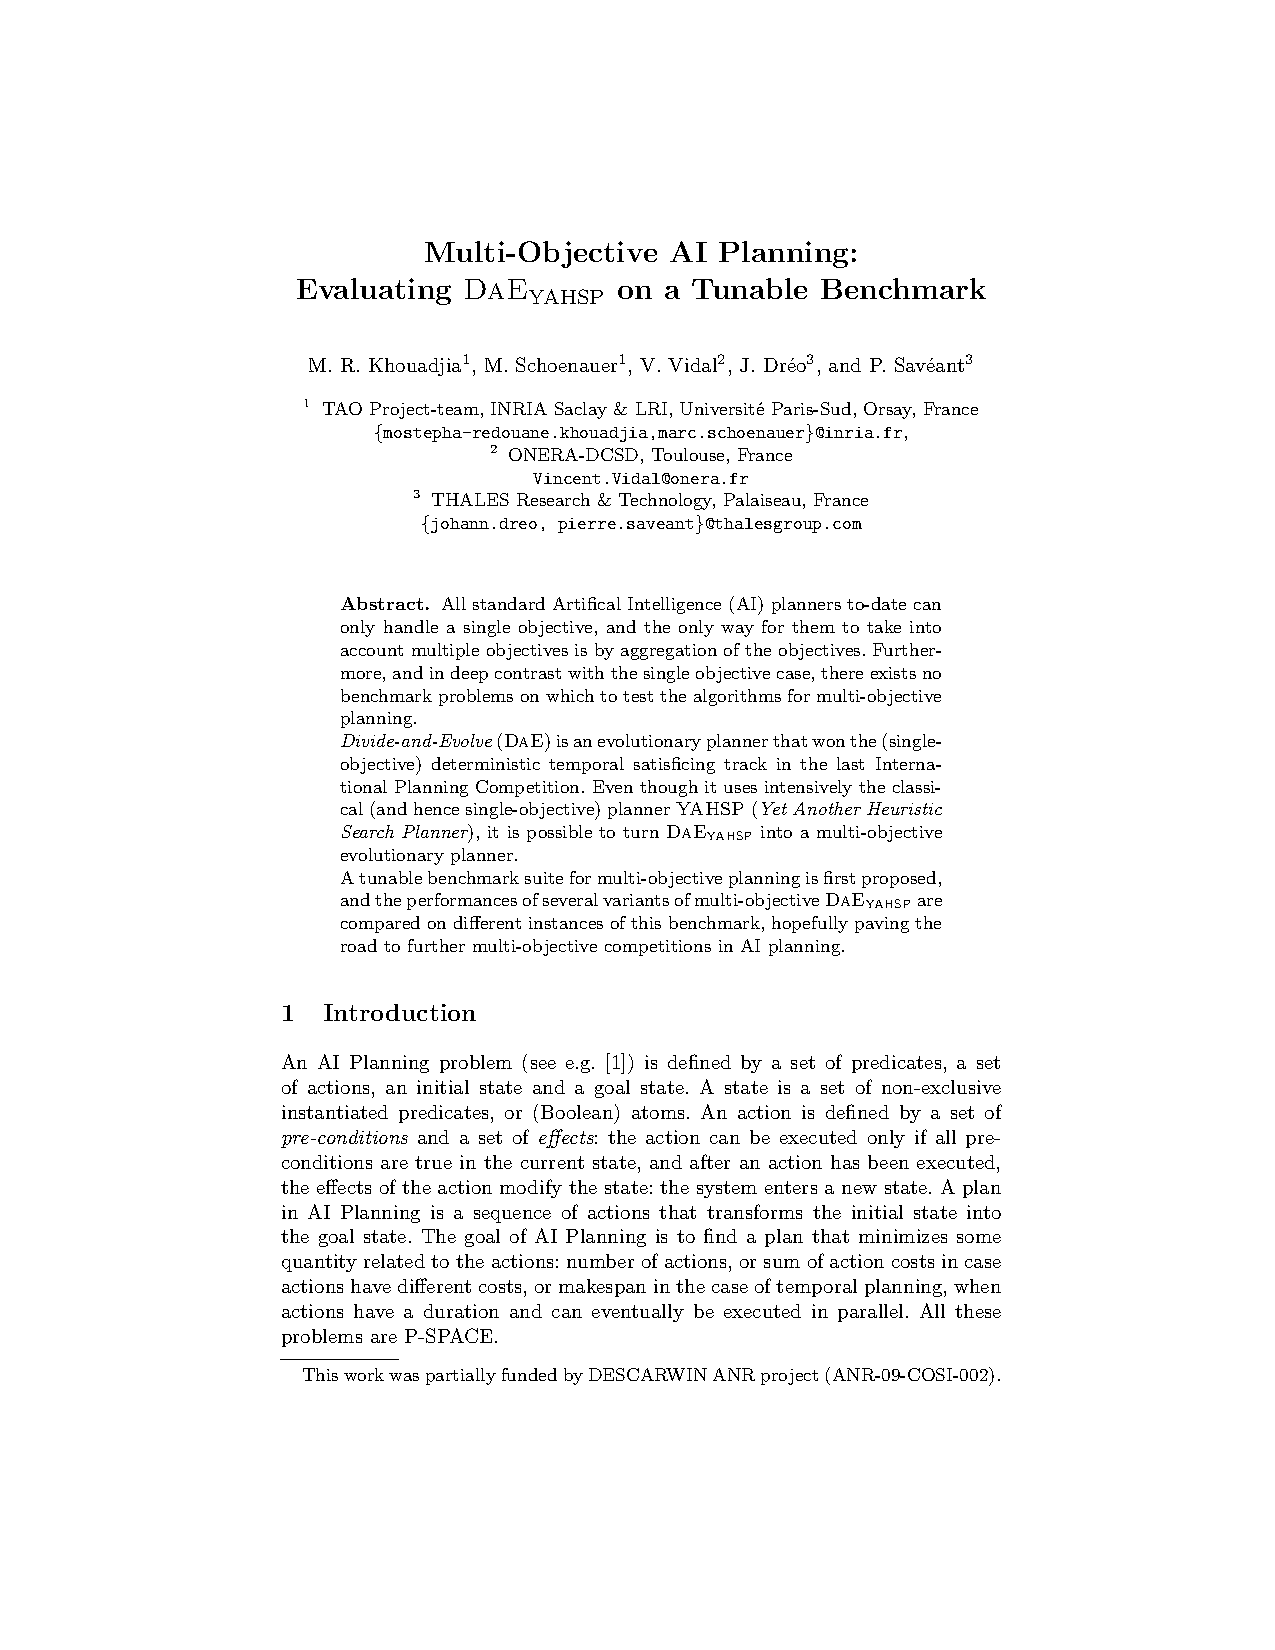
\includepdf[height=32cm,pages=-,offset=0cm -4cm]{emo2012.pdf}
\newpage
\hoffset -2cm

\chapter{Comparing Aggregation and Pareto Approaches}

\newpage
\hoffset 0cm
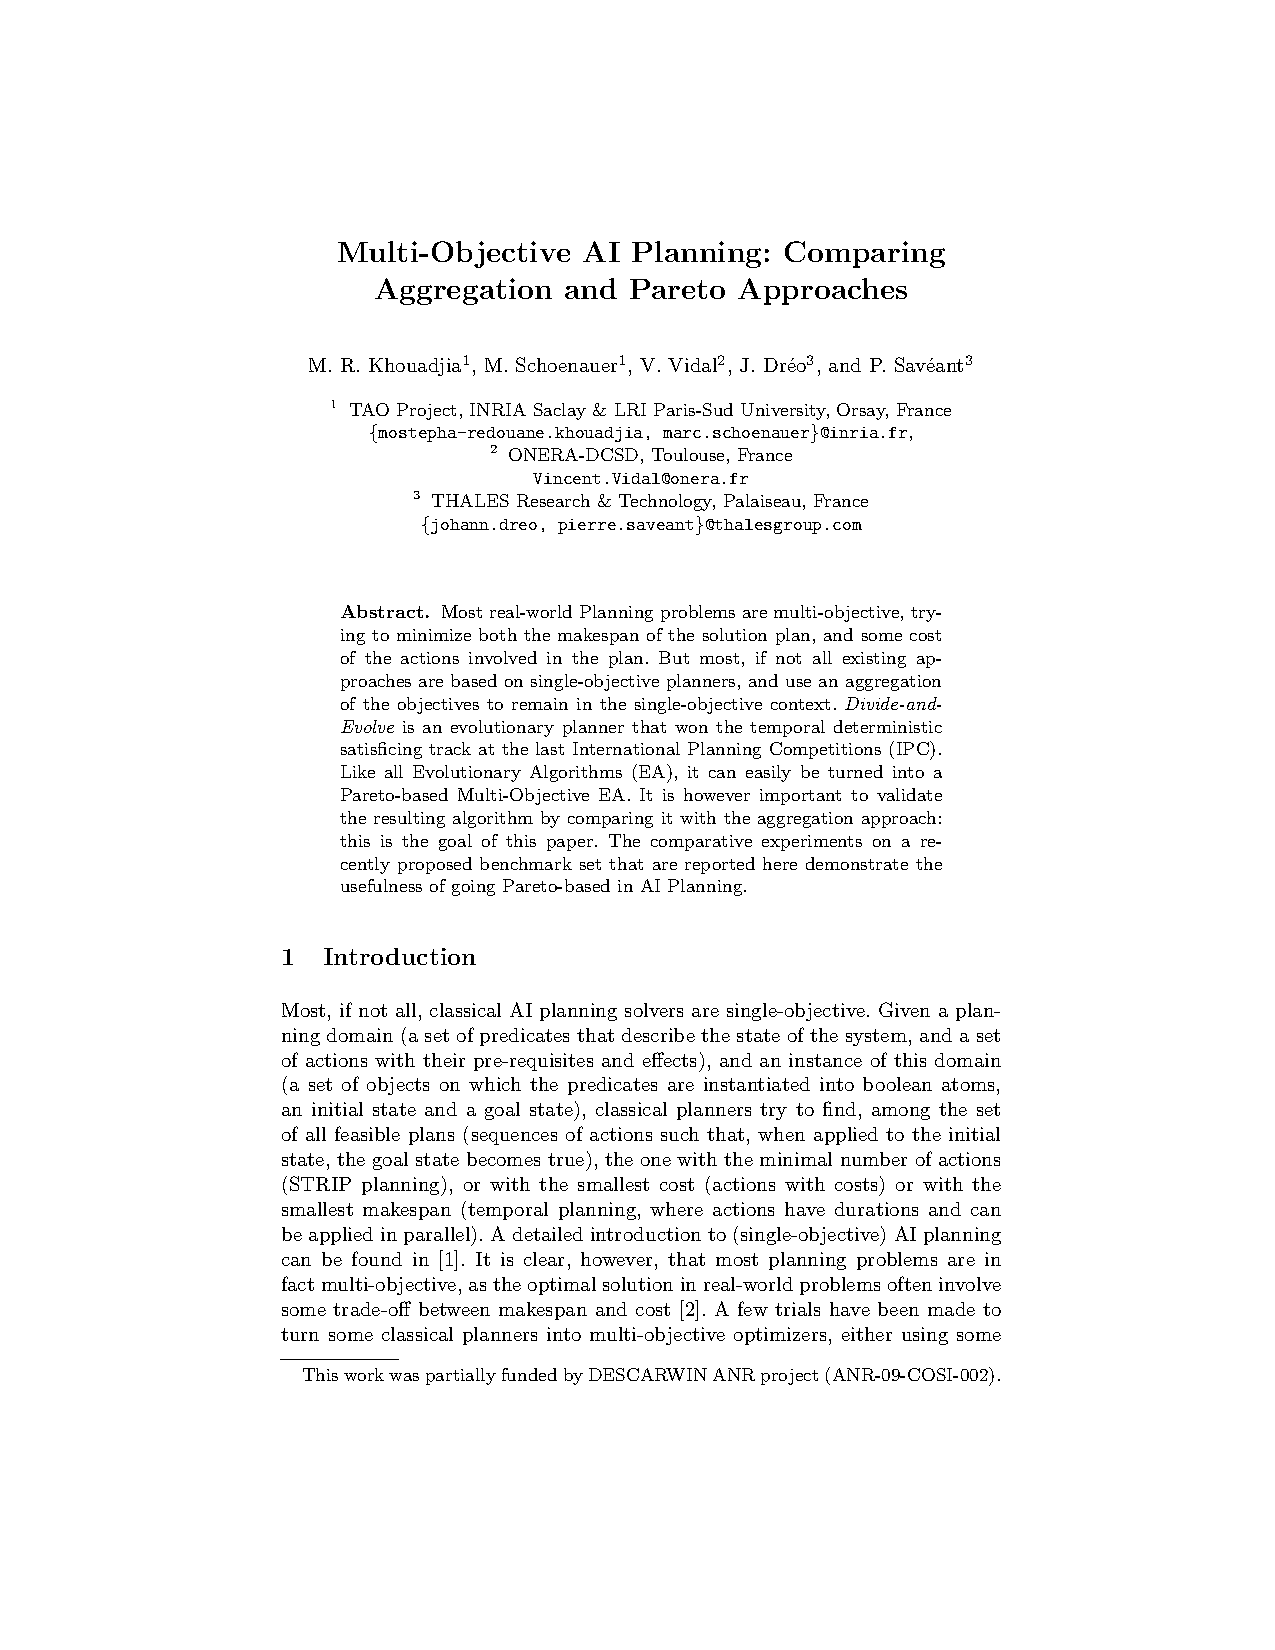
\includepdf[height=32cm,pages=-,offset=0cm -4cm]{evocop2012.pdf}
\newpage
\hoffset -2cm

\chapter{Comparing Metric-Sensitive and Pareto Approaches}

\newpage
\hoffset 0cm
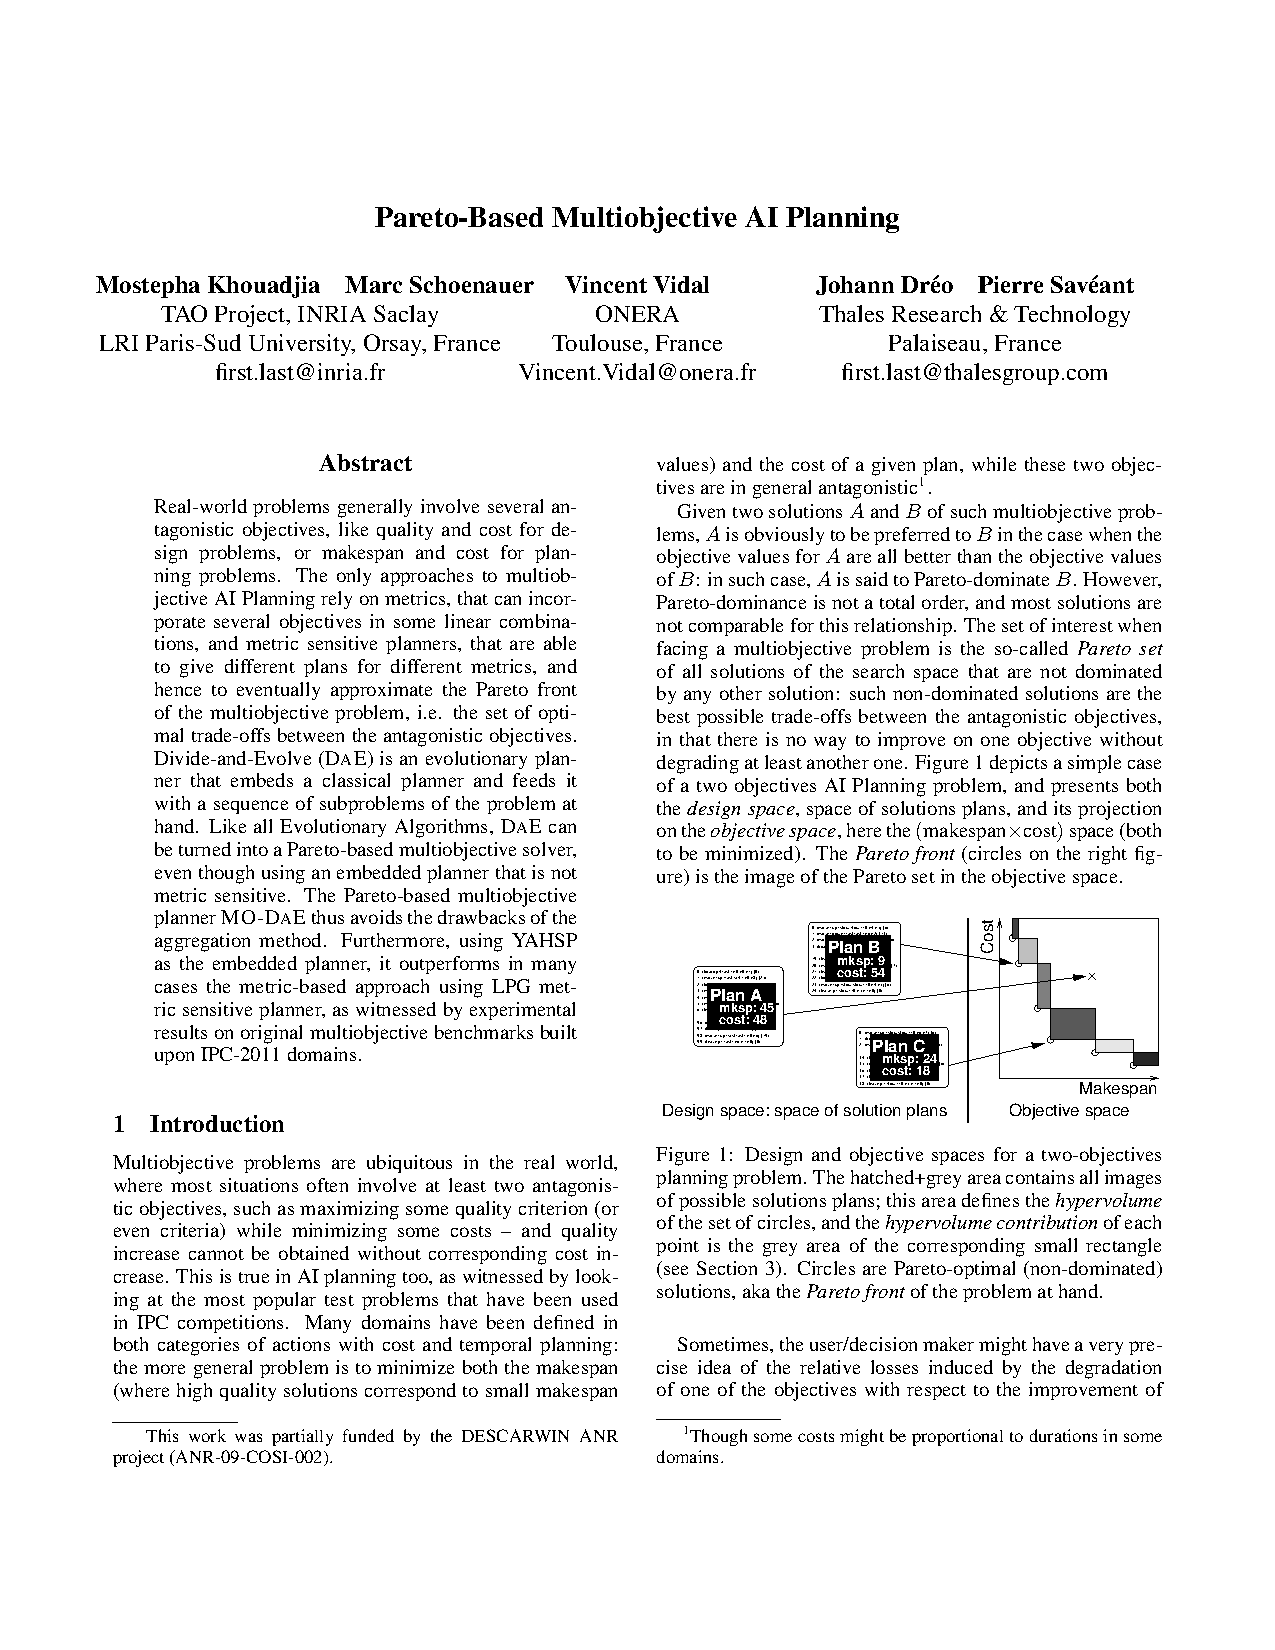
\includepdf[width=22.5cm,height=32cm,pages=-,offset=0cm -4cm]{567.pdf}
\hoffset -2cm


\end{document}